% =====================================================================================================
% Appendix: experimental details (A), additional results (B), analysis of probe relocation (C),
% example maps (D) and key code (E). Every part supports a statement of the main text.
% =====================================================================================================

\counterwithin{figure}{section}
\counterwithin{table}{section}
\captionsetup{skip=5pt}
\raggedbottom

\section{Experimental details}
\label{app:setup}

\paragraph{Models.} All models are frozen ViTs with $16{\times}16$ patches on $224{\times}224$ inputs, taken from timm~\citep{wightman2019}. \emph{DeiT-S and DeiT-B}~\citep{touvron2021}: \texttt{deit\_small\_patch16\_224.fb\_in1k} and \texttt{deit\_base\_patch16\_224.fb\_in1k} (resize to 248, centre crop 224: a crop ratio of 0.9). \emph{DINO ViT-S/16}~\citep{caron2021}: \texttt{vit\_small\_patch16\_224.dino} with the official DINO linear head (resize to 256, centre crop 224: a crop ratio of 0.875). \emph{DeiT-S with a test-time register}~\citep{jiang2025}: the activations of eight feed-forward units in layers 4 and 5 are moved to one added register token, which is left out of every map, like CLS. The units were selected on 500 ImageNet-S images, where they reduce the number of high-norm patch tokens (counted per layer) by 92.75\% and keep 99.0\% of the predictions; on the other 11,919 images the reduction is 91.5\%, and ImageNet accuracy stays at 79.8\%. For DeiT-B the same search found no such units (44.9\% reduction with 32 units), so we report the register for DeiT-S only. \emph{Top-$k$ training}: the DeiT-S checkpoint released with MiTA~\citep{wen2026mita} (25 summary slots, $k=25$), with its own preprocessing (crop ratio 0.875). It differs from our DeiT-S in training and preprocessing, so its row in Table~\ref{tab:main} is not a controlled comparison; its deletion score is undefined because its summary slots pool fixed regions of the full grid. Both model-side fixes are tested at size S only; in a preliminary comparison with an earlier protocol, top-$k$ training scored 0.011 lower in object enrichment than its baseline at size S but 0.037 higher at size Tiny, so the result should not be read beyond DeiT-S.

\paragraph{Data.} \emph{Execution test}: 5,000 randomly drawn ImageNet validation images~\citep{deng2009}. \emph{ImageNet-S}~\citep{gao2023}: all 12,419 validation images with segmentation masks; enrichment is defined for 12,150 of them (12,144 for DINO ViT-S), after excluding images without valid foreground or background patches, and deletion uses a random subset of 2,000. \emph{ClickMe}~\citep{linsley2019,fel2022}: 17,408 images with human importance maps. Images are resized from $256{\times}256$ to $224{\times}224$ without cropping; heatmaps are resized to $64{\times}64$, blurred with a $10{\times}10$ Gaussian ($\sigma=10$), then resized to $224{\times}224$. \emph{Held-out set}: 4,000 ImageNet validation images excluded from map-quality and execution evaluation; 2,000 train the position probes, and the other 2,000 give the mean maps, the probe accuracies and the blur widths. While building this set we found that only 2 of 4,002 candidate validation images matched a ClickMe image, so the ClickMe images are very likely ImageNet training images, which all three models have seen.

\paragraph{Diagnostics.} All three are computed per layer. \emph{Specificity}: with $\bar s$ the mean received-attention map of the held-out images and $\operatorname{Var}_j$ the variance over the 196 patches of one image, the share explained is $1-\sum_x\operatorname{Var}_j(s-\bar s)\,/\sum_x\operatorname{Var}_j(s)$, summed over the ImageNet-S images $x$. \emph{Location}: the top-1 accuracy of the linear position probe on the 196 patch tokens of each of 2,000 held-out images. \emph{Contribution}: the share of received attention on high-norm tokens, on the ImageNet-S images. The high-norm threshold (three times the median, defined below) is an operational definition fixed before the experiments; we did not test other thresholds. The correction itself uses no threshold.

\paragraph{Corrections and matched controls.} All are applied per layer and then summed over layers 9--12; queries run over all 197 tokens and maps cover the 196 patches.
\emph{Mean-map subtraction} subtracts the model's mean received-attention map over the 2,000 held-out images. Its control subtracts a centred isotropic Gaussian ($\sigma=3.5$ patches) scaled to the spatial standard deviation of that mean map; it is exactly radial.
\emph{Probe relocation} uses one linear 196-way classifier per model and layer (36 in all) on the standardised tokens after the block's first layer norm (Adam, learning rate 0.01, 30 epochs) and computes $r_p=\sum_j s_j P_\ell(p\mid x_j)$, which keeps the total score. Its control is a Gaussian blur whose width is set so that it moves the score as far, in mean squared displacement, as relocation does on held-out tokens of that layer (0.7--2.9 patches).
\emph{Contribution weighting} computes $c_j=\sum_h\sum_i a_{ij}^h\lVert W_O^h v_j^h\rVert_2$, where $W_O^h$ is the head's slice of the output projection; $a_{ij}^h\lVert W_O^h v_j^h\rVert$ is the per-head norm of \citet{kobayashi2020}. A \emph{high-norm token} is a patch whose block input has a norm above three times the image's median patch norm in that layer; the control sets received attention to zero at these patches.
\emph{All three corrections}: contribution weighting, then probe relocation, then subtraction of the held-out mean of the resulting map.

\paragraph{Metrics.} \emph{Same-ring object enrichment.} A patch is valid if it contains at least one non-ignored pixel, and is an object patch if at least half of its non-ignored pixels belong to the image's class mask. We select as many top-scoring patches as there are object patches. For every ring of patches at the same distance from the grid centre, we take the object rate among its selected patches minus that among all its patches, and average over rings, weighted by their selected patches. Invalid patches are excluded from selection and ring baselines. Ties are broken with the fixed seeded perturbation used in the original runs. A purely radial map scores zero in expectation over tie-breaking.
\emph{Image-specific ClickMe alignment.} The map is upsampled to $224{\times}224$ and correlated (Spearman, over pixels) with the image's own human map; we subtract its correlation with the previous image's human map within each batch (\texttt{roll(1)}; batch size 64). For an image-independent map, these differences average to zero over the paired set because the control permutes the same human maps; individual-image differences need not be zero. This removes fixed-prior alignment on average, without guaranteeing invariance to a prior mixed into an image-dependent map.
\emph{Deletion faithfulness.} Patches are removed in the order of the map by dropping their tokens; at budgets of 0 to 147 patches we record whether the top-1 class is unchanged. The score is the symmetric relevance gain of \citet{bluecher2024}: the area under the least-important-first curve minus that under the most-important-first curve.
\emph{Validity of the metrics.} A random map, a centred Gaussian and the mean map all score within 0.004 of zero on enrichment and on ClickMe alignment (the two image-independent maps have exactly zero mean on the latter, up to numerical precision); on deletion the centred Gaussian scores 0.110, 0.099 and 0.140 (DeiT-S, DeiT-B, DINO ViT-S), which is why every correction is compared with a matched control.
\emph{Statistics.} One value per image; paired bootstrap over images (1,000 resamples, 95\% percentile intervals). A difference is \emph{higher} (\textit{h}) or \emph{lower} (\textit{l}) if its interval excludes zero and its size exceeds 0.02 (0.05 for deletion), and \emph{comparable} (\textit{c}) otherwise. The registered rule and margins are unchanged: comparable combines intervals containing zero with effects below the margin and is not a formal equivalence claim. Intervals are not adjusted for multiple comparisons; the practical margin does not itself provide multiplicity control.

\paragraph{Registered predictions.} Before the formal runs we fixed the definitions above, the margins, the comparisons of Table~\ref{tab:main} and the predictions of Table~\ref{tab:app-registered}; the record is the file \texttt{docs/preregistration.md} of the repository. R2 was registered with three possible verdicts: holds (four of four cells), partly holds (one to three) and does not hold (none). For each correction against its control, the comparison was fixed without a direction. Earlier runs of the execution test and of the diagnostics had been seen, so the last two rows are replications. Other analyses are marked post hoc.

\begin{table}[!htbp]
\caption{Registered predictions and outcomes (centre-controlled metrics: enrichment and ClickMe alignment).}
\label{tab:app-registered}
\centering\footnotesize
\setlength{\tabcolsep}{4pt}
\begin{tabular}{@{}l>{\raggedright\arraybackslash}p{3.55in}>{\raggedright\arraybackslash}p{1.35in}@{}}
\toprule
 & Prediction & Outcome\\
\midrule
R1 & Contribution weighting is comparable to received attention in DINO ViT-S on all three metrics & holds (3 of 3 cells)\\
R1 & Relocation at layers 1--4 is comparable to received attention on the centre-controlled metrics in all models & holds (6 of 6 cells)\\
R2 & All three corrections together are higher than received attention on the centre-controlled metrics in DeiT-S and DeiT-B & partly holds (1 of 4 cells: DeiT-B, ClickMe)\\
R3 & Neither model-side change is higher than DeiT-S received attention on the centre-controlled metrics & holds (4 of 4 cells)\\
\midrule
-- & Execution agreement rises with $k$ and exceeds that of random sets at every $k$ & holds in all models\\
-- & Probe accuracy falls with depth; the share of attention on high-norm tokens peaks in layers 6--12 of the supervised models and is below 1\% in every layer of DINO ViT-S & holds in all models\\
\bottomrule
\end{tabular}
\end{table}

\paragraph{Compute and code.} All experiments took about 19 GPU hours on NVIDIA L4 GPUs. Code and result tables: \url{https://github.com/hhuang999/vit-fastweight-lens}.

% =====================================================================================================
\section{Additional results}
\label{app:more}
\suppressfloats[t]

\noindent\begin{minipage}[t]{3.15in}
\paragraph{Execution test.} The $14{\times}14$ grid is pooled into 16 overlapping regions. In every layer and head, each region's mean query is scored against all keys, and its $k$ highest-scoring keys form the region's reading set (the CLS query keeps its own top-$k$ set). The sets come from one pass of the unmodified model. We then rerun the model with every query restricted to its region's set, in all 12 layers at once, and record whether the top-1 class is unchanged. Figure~\ref{fig:app-ksweep} shows that top-$k$ sets beat random sets of the same size at every $k$ from 4 to 128 in all three models, and that agreement rises with $k$. The dotted line alone was run with a crop ratio of 0.875 for all models (0.9 for DeiT-S and DeiT-B elsewhere).
\end{minipage}\hfill
\begin{minipage}[t]{2.25in}
\vspace{2pt}
\centering
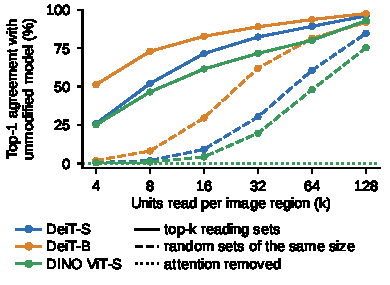
\includegraphics[width=2.1in]{execution_k_sweep}
\captionof{figure}{Top-1 agreement with the unmodified model when queries read only top-$k$ units (solid), random units (dashed) or nothing (dotted). 95\% intervals: at most $\pm1.5$ points.}
\label{fig:app-ksweep}
\end{minipage}

\paragraph{Diagnostics per layer.} Table~\ref{tab:app-diag} lists the values plotted in Fig.~\ref{fig:diag}. Two numbers of the main text are not in the table. First, in layers 9--12, 82--98\% of the variance of the mean map is explained by the distance from the grid centre. Second, averaged over layers 9--12, the mean value-vector norm $\lVert v_j\rVert$ of high-norm tokens is 0.29 (DeiT-S) and 0.23 (DeiT-B) times the median of the other patches (measured on 11,919 ImageNet-S images using uniform crop ratio 0.875, unlike the main DeiT evaluation at 0.9).

\paragraph{Recovery at the last layer.} In the supervised models, single-layer received attention is worse at layer 12 than at the best of layers 8--11 (Fig.~\ref{fig:diag}d). Applied to layer 12, contribution weighting recovers 62\% and 33\% of this drop on enrichment (DeiT-S, DeiT-B), 31\% and 45\% on ClickMe alignment, and 8\% and 29\% on deletion. The other two corrections make layer 12 worse.

\begin{table}[!htbp]
\caption{Diagnostics per layer, as plotted in Fig.~\ref{fig:diag} (S, B, D: DeiT-S, DeiT-B, DINO ViT-S; probe chance: 0.5\%).}
\label{tab:app-diag}
\centering
% Per-layer diagnostics, generated from results/diagnose.csv by diag_table.py.
\footnotesize
\setlength{\tabcolsep}{2.6pt}
\begin{tabular}{r >{\centering\arraybackslash}p{0.8cm} >{\centering\arraybackslash}p{0.8cm} >{\centering\arraybackslash}p{0.8cm} >{\centering\arraybackslash}p{0.8cm} >{\centering\arraybackslash}p{0.8cm} >{\centering\arraybackslash}p{0.8cm} >{\centering\arraybackslash}p{0.8cm} >{\centering\arraybackslash}p{0.8cm} >{\centering\arraybackslash}p{0.8cm} >{\centering\arraybackslash}p{1.05cm} >{\centering\arraybackslash}p{1.05cm} >{\centering\arraybackslash}p{1.05cm}}
\toprule
 & \multicolumn{3}{c}{\makecell{Specificity:\\mean-map share (\%)}} & \multicolumn{3}{c}{\makecell{Location:\\probe accuracy (\%)}} & \multicolumn{3}{c}{\makecell{Contribution:\\high-norm share (\%)}} & \multicolumn{3}{c}{\makecell{Map quality:\\ClickMe alignment}} \\
\cmidrule(lr){2-4}\cmidrule(lr){5-7}\cmidrule(lr){8-10}\cmidrule(lr){11-13}
Layer & S & B & D & S & B & D & S & B & D & S & B & D \\
\midrule
1 & 6.8 & 12.4 & 11.2 & 100.0 & 100.0 & 99.9 & 0.0 & 0.0 & 0.0 & $-$0.108 & $-$0.111 & $-$0.089 \\
2 & 21.2 & 14.0 & 7.4 & 100.0 & 100.0 & 100.0 & 0.0 & 0.0 & 0.0 & 0.007 & 0.041 & 0.064 \\
3 & 13.7 & 15.0 & 19.7 & 99.9 & 100.0 & 99.9 & 0.0 & 0.0 & 0.0 & 0.081 & 0.004 & 0.056 \\
4 & 6.9 & 7.5 & 14.6 & 99.0 & 100.0 & 99.8 & 0.0 & 0.0 & 0.0 & 0.132 & 0.110 & 0.140 \\
5 & 7.8 & 5.8 & 14.6 & 97.5 & 99.9 & 99.6 & 0.1 & 0.0 & 0.0 & 0.148 & 0.130 & 0.150 \\
6 & 5.2 & 6.2 & 11.9 & 85.3 & 99.5 & 98.9 & 2.6 & 0.0 & 0.0 & 0.136 & 0.151 & 0.167 \\
7 & 4.4 & 5.4 & 12.4 & 65.0 & 96.8 & 95.9 & 7.4 & 3.5 & 0.0 & 0.147 & 0.131 & 0.150 \\
8 & 4.2 & 5.4 & 6.6 & 43.9 & 91.8 & 85.6 & 9.3 & 12.9 & 0.0 & 0.149 & 0.118 & 0.170 \\
9 & 4.2 & 5.7 & 9.5 & 31.0 & 83.6 & 67.4 & 9.3 & 21.5 & 0.0 & 0.184 & 0.112 & 0.198 \\
10 & 4.3 & 5.5 & 15.2 & 23.1 & 66.8 & 50.5 & 9.1 & 28.1 & 0.0 & 0.171 & 0.139 & 0.207 \\
11 & 4.1 & 5.8 & 16.7 & 19.4 & 49.2 & 39.2 & 5.6 & 43.5 & 0.0 & 0.149 & 0.120 & 0.211 \\
12 & 3.3 & 5.0 & 13.6 & 18.1 & 31.8 & 35.7 & 7.2 & 22.2 & 0.0 & 0.098 & 0.023 & 0.179 \\
\bottomrule
\end{tabular}

\end{table}

\begin{table}[!tbp]
\caption{Paired differences, layers 9--12: mean with 95\% paired-bootstrap interval and verdict (\textit{h} higher, \textit{c} comparable, \textit{l} lower). Top: against received attention. Bottom: each correction against its matched control.}
\label{tab:app-paired}
\centering
% Paired differences: blocks copied verbatim from repo/paper/tables/appendix/paired_differences.tex by
% make/make_paired_table.py (titles simplified, numbers unchanged).
\footnotesize
\setlength{\tabcolsep}{4pt}
\renewcommand{\arraystretch}{0.92}
\begin{tabular}{lccc}
\toprule
Model & Same-ring enrichment & ClickMe alignment & Deletion faithfulness \\
\midrule
\multicolumn{4}{l}{\textit{Contribution weighting $-$ received attention}} \\
DeiT-S & 0.038 {\scriptsize [0.036, 0.039]}\,\textit{h} & 0.033 {\scriptsize [0.032, 0.034]}\,\textit{h} & 0.017 {\scriptsize [0.013, 0.021]}\,\textit{c} \\
DeiT-B & 0.065 {\scriptsize [0.063, 0.067]}\,\textit{h} & 0.058 {\scriptsize [0.056, 0.059]}\,\textit{h} & 0.029 {\scriptsize [0.024, 0.034]}\,\textit{c} \\
DINO ViT-S & $-$0.004 {\scriptsize [$-$0.004, $-$0.003]}\,\textit{c} & $-$0.001 {\scriptsize [$-$0.001, $-$0.001]}\,\textit{c} & 0.000 {\scriptsize [$-$0.003, 0.004]}\,\textit{c} \\
\addlinespace[2pt]
\multicolumn{4}{l}{\textit{Mean-map subtraction $-$ received attention}} \\
DeiT-S & $-$0.002 {\scriptsize [$-$0.003, $-$0.002]}\,\textit{c} & 0.009 {\scriptsize [0.008, 0.010]}\,\textit{c} & $-$0.028 {\scriptsize [$-$0.034, $-$0.023]}\,\textit{c} \\
DeiT-B & $-$0.003 {\scriptsize [$-$0.004, $-$0.003]}\,\textit{c} & $-$0.020 {\scriptsize [$-$0.021, $-$0.019]}\,\textit{l} & $-$0.025 {\scriptsize [$-$0.031, $-$0.019]}\,\textit{c} \\
DINO ViT-S & 0.002 {\scriptsize [0.001, 0.003]}\,\textit{c} & 0.044 {\scriptsize [0.040, 0.048]}\,\textit{h} & $-$0.052 {\scriptsize [$-$0.059, $-$0.044]}\,\textit{l} \\
\addlinespace[2pt]
\multicolumn{4}{l}{\textit{Probe relocation $-$ received attention}} \\
DeiT-S & $-$0.099 {\scriptsize [$-$0.101, $-$0.097]}\,\textit{l} & $-$0.073 {\scriptsize [$-$0.076, $-$0.069]}\,\textit{l} & $-$0.161 {\scriptsize [$-$0.171, $-$0.150]}\,\textit{l} \\
DeiT-B & $-$0.054 {\scriptsize [$-$0.055, $-$0.052]}\,\textit{l} & $-$0.057 {\scriptsize [$-$0.059, $-$0.055]}\,\textit{l} & $-$0.118 {\scriptsize [$-$0.127, $-$0.110]}\,\textit{l} \\
DINO ViT-S & $-$0.115 {\scriptsize [$-$0.117, $-$0.113]}\,\textit{l} & $-$0.064 {\scriptsize [$-$0.067, $-$0.062]}\,\textit{l} & $-$0.144 {\scriptsize [$-$0.153, $-$0.134]}\,\textit{l} \\
\addlinespace[2pt]
\multicolumn{4}{l}{\textit{All three corrections $-$ received attention}} \\
DeiT-S & $-$0.081 {\scriptsize [$-$0.083, $-$0.079]}\,\textit{l} & $-$0.034 {\scriptsize [$-$0.038, $-$0.030]}\,\textit{l} & $-$0.160 {\scriptsize [$-$0.171, $-$0.149]}\,\textit{l} \\
DeiT-B & $-$0.001 {\scriptsize [$-$0.003, 0.001]}\,\textit{c} & 0.030 {\scriptsize [0.027, 0.032]}\,\textit{h} & $-$0.084 {\scriptsize [$-$0.093, $-$0.076]}\,\textit{l} \\
DINO ViT-S & $-$0.111 {\scriptsize [$-$0.114, $-$0.109]}\,\textit{l} & $-$0.031 {\scriptsize [$-$0.035, $-$0.027]}\,\textit{l} & $-$0.195 {\scriptsize [$-$0.205, $-$0.184]}\,\textit{l} \\
\midrule
\multicolumn{4}{l}{\textit{Contribution weighting $-$ zero high-norm tokens (its control)}} \\
DeiT-S & 0.026 {\scriptsize [0.025, 0.027]}\,\textit{h} & 0.022 {\scriptsize [0.021, 0.023]}\,\textit{h} & 0.012 {\scriptsize [0.008, 0.016]}\,\textit{c} \\
DeiT-B & 0.025 {\scriptsize [0.024, 0.026]}\,\textit{h} & 0.017 {\scriptsize [0.016, 0.018]}\,\textit{c} & 0.013 {\scriptsize [0.008, 0.018]}\,\textit{c} \\
DINO ViT-S & $-$0.004 {\scriptsize [$-$0.004, $-$0.003]}\,\textit{c} & $-$0.001 {\scriptsize [$-$0.001, $-$0.001]}\,\textit{c} & 0.000 {\scriptsize [$-$0.003, 0.004]}\,\textit{c} \\
\addlinespace[2pt]
\multicolumn{4}{l}{\textit{Mean-map subtraction $-$ centre-Gaussian subtraction (its control)}} \\
DeiT-S & 0.005 {\scriptsize [0.004, 0.005]}\,\textit{c} & $-$0.003 {\scriptsize [$-$0.005, $-$0.001]}\,\textit{c} & 0.040 {\scriptsize [0.034, 0.047]}\,\textit{c} \\
DeiT-B & 0.022 {\scriptsize [0.021, 0.023]}\,\textit{h} & 0.025 {\scriptsize [0.020, 0.030]}\,\textit{h} & 0.120 {\scriptsize [0.109, 0.130]}\,\textit{h} \\
DINO ViT-S & 0.001 {\scriptsize [0.001, 0.002]}\,\textit{c} & $-$0.001 {\scriptsize [$-$0.001, 0.000]}\,\textit{c} & 0.001 {\scriptsize [$-$0.003, 0.005]}\,\textit{c} \\
\addlinespace[2pt]
\multicolumn{4}{l}{\textit{Probe relocation $-$ matched blur (its control)}} \\
DeiT-S & $-$0.054 {\scriptsize [$-$0.056, $-$0.051]}\,\textit{l} & $-$0.068 {\scriptsize [$-$0.073, $-$0.064]}\,\textit{l} & $-$0.105 {\scriptsize [$-$0.116, $-$0.095]}\,\textit{l} \\
DeiT-B & 0.035 {\scriptsize [0.034, 0.036]}\,\textit{h} & $-$0.018 {\scriptsize [$-$0.020, $-$0.015]}\,\textit{c} & $-$0.047 {\scriptsize [$-$0.055, $-$0.037]}\,\textit{c} \\
DINO ViT-S & $-$0.105 {\scriptsize [$-$0.107, $-$0.102]}\,\textit{l} & $-$0.083 {\scriptsize [$-$0.085, $-$0.080]}\,\textit{l} & $-$0.146 {\scriptsize [$-$0.155, $-$0.137]}\,\textit{l} \\
\bottomrule
\end{tabular}

\end{table}

\paragraph{Differences behind Table~\ref{tab:main}.} Table~\ref{tab:app-paired} gives the paired differences with their intervals. The values in Table~\ref{tab:main} have 95\% intervals of at most $\pm0.005$ on enrichment and ClickMe alignment and $\pm0.012$ on deletion. The model-side differences from DeiT-S received attention are $+0.012$ [$0.011$, $0.013$] on enrichment, $+0.013$ [$0.012$, $0.013$] on ClickMe and $0.000$ [$-0.005$, $0.004$] on deletion for the test-time register, and $-0.040$ [$-0.042$, $-0.039$] and $-0.042$ [$-0.044$, $-0.040$] on the first two for top-$k$ training.

\paragraph{Tests of the contribution account.} Contribution weighting should work by down-weighting tokens that receive attention but contribute little. One consequence was registered (R1), and two further tests were added post hoc. \emph{No practically meaningful gain in DINO (R1).} In DINO ViT-S, where no attention falls on high-norm tokens, every difference from received attention is at most 0.004 in size (Table~\ref{tab:app-paired}). \emph{More high-norm attention, more gain (post hoc).} Across images, gains have a weak positive association with the share of received attention on high-norm tokens: Spearman $+0.075$ [$0.057$, $0.092$] and $+0.132$ [$0.113$, $0.150$] on enrichment (DeiT-S, DeiT-B), $+0.045$ [$0.032$, $0.060$] and $+0.158$ [$0.143$, $0.173$] on ClickMe. \emph{The weights must match the tokens (post hoc).} Against the same weights shuffled among the patches of each head, contribution weighting is higher in all four supervised cells: $+0.038$ [$0.037$, $0.040$] and $+0.073$ [$0.071$, $0.076$] on enrichment, $+0.035$ [$0.035$, $0.036$] and $+0.067$ [$0.065$, $0.068$] on ClickMe. Finally, also post hoc, weighting by $\lVert v_j^h\rVert$ instead of $\lVert W_O^h v_j^h\rVert$ is comparable in every cell (differences $-0.010$ to $0.000$): in practice the correction is the value-norm weighting of \citet{kobayashi2020} and \citet{zhu2024}.

% =====================================================================================================
\section{Why does probe relocation fail?}
\label{app:reloc}

Relocation lowers every deep-layer cell (Table~\ref{tab:main}). Two planned comparisons narrow the problem. Where the probe is accurate, relocation is harmless (R1): at layers 1--4 it changes enrichment and ClickMe alignment by at most 0.004 in every model. And in DeiT-S and DINO ViT-S it is lower than a blur that moves the score equally far (Table~\ref{tab:app-paired}). The rest of this section is post hoc: Table~\ref{tab:app-reloc} lists four explanations that we tested after seeing this result; none meets its specified criterion. Most probability lies near the true patch, and replacing the linear probe with the tested MLP does not restore map quality. This does not exclude all probe-capacity or calibration limitations. The probe targets index decodability rather than input-content provenance; whether this mismatch explains the failed relocation remains untested (Section~\ref{sec:exp}).

\begin{table}[!htbp]
\caption{Four explanations for the failure of probe relocation, and their tests (post hoc). Cells are the two centre-controlled metrics in the three models.}
\label{tab:app-reloc}
\centering
% Four candidate explanations for the failure of probe relocation, each with its test and result.
% Written for the paper from results/c2_analysis/ and results/supplementary/ (mlp_probe.csv, globalisation.csv)
% as summarised in paper/evidence_dossier.md; no number is computed here.
\footnotesize
\setlength{\tabcolsep}{4pt}
\renewcommand{\arraystretch}{1.08}
\begin{tabular}{>{\raggedright\arraybackslash}p{3.1cm}>{\raggedright\arraybackslash}p{4.9cm}>{\raggedright\arraybackslash}p{5.1cm}}
\toprule
Explanation & Test (layers 9--12 unless stated) & Result \\
\midrule
The probe sends score to distant, wrong patches & Share of the probe's error mass more than three patches from the true patch & Small: 2--29\% across models and layers. At layer 12, 45\%, 66\% and 81\% of the probability lies within the $3{\times}3$ neighbourhood of the true patch \\
The probe has a fixed position preference & Peak of the probe's mean prediction relative to uniform; its correlation with the mean map & Close to uniform (peak 1.1--1.3 times the uniform value); at most weakly related to the mean map \\
The linear probe is too weak & Two-layer MLP probe in place of the linear one & Accuracy at layer 12 rises by only 1.8, 3.8 and 6.7 points; relocation with the MLP probe is still lower than received attention in all six cells \\
Global tokens are harder to place & Probe accuracy and entropy against a token's similarity to the image's mean token (layers 10--12) & No consistent relation; accuracy falls with globality only in DeiT-B \\
\bottomrule
\end{tabular}

\end{table}

% =====================================================================================================
\section{Example maps}
\label{app:gallery}

The stored gallery holds 24 ClickMe images drawn at random with a fixed seed. Fig.~\ref{fig:app-gallery-first} shows the two with the smallest ClickMe index (the original v8 main-text examples), and Fig.~\ref{fig:app-gallery} the next four. The image-selection rule is unchanged. Received attention and contribution weighting look much alike, while probe relocation spreads the score over many more patches. The gains in Table~\ref{tab:main} are averages of small changes in how each map ranks its patches, which single maps do not show.

\begin{figure}[!htbp]
\centering
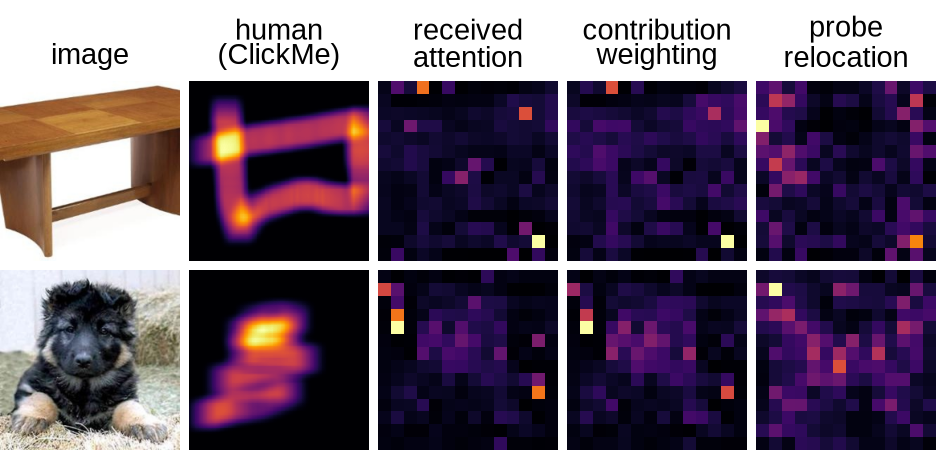
\includegraphics[width=4.7in]{example_maps}
\caption{The first two fixed-seed examples, DeiT-S, layers 9--12. Each map is min--max normalised; these images were not selected for correction gain.}
\label{fig:app-gallery-first}
\end{figure}

\begin{figure}[!htbp]
\centering
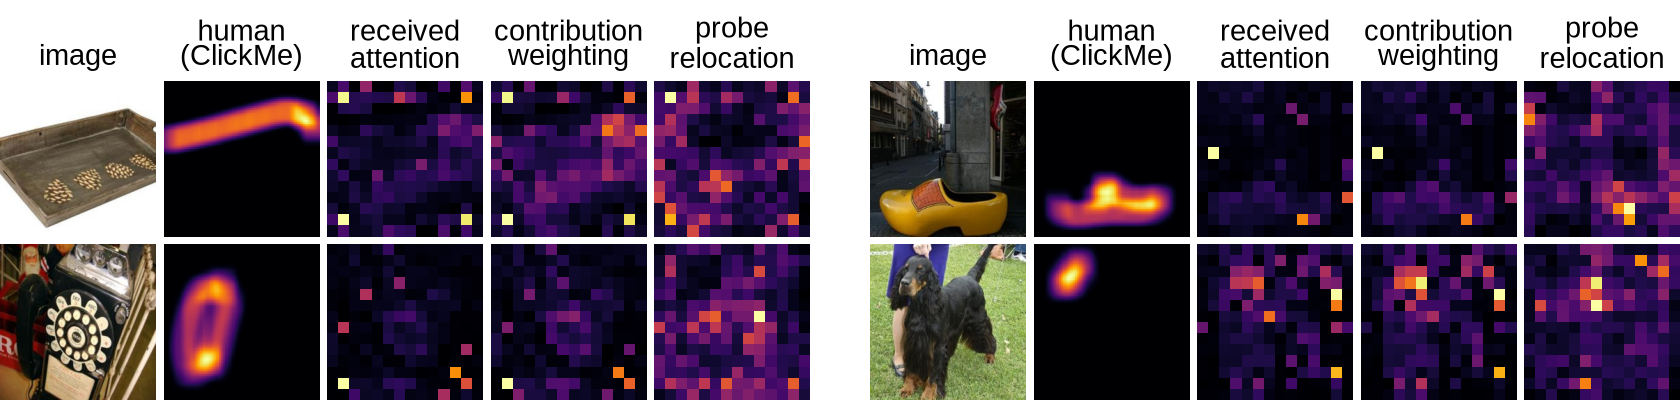
\includegraphics[width=5.5in]{example_maps_more}
\caption{DeiT-S on four further ClickMe images, layers 9--12; each map is min--max normalised.}
\label{fig:app-gallery}
\end{figure}

% =====================================================================================================
\section{Key parts of the code}
\label{app:code}

Given the attention $a_{ij}^h$ and values $v_j^h$ of a layer, the readings are:

\begin{lstlisting}[language=Python]
def received_and_contribution(p, v, w_o, prefix=1):
    # p: [B,H,N,N] attention a_ij^h (queries i, keys j); v: [B,H,N,d] values; w_o: [D,H,d] W_O by head
    gram = torch.einsum('dhe,dhf->hef', w_o, w_o)                 # W_O^h^T W_O^h
    length = torch.einsum('bhne,hef,bhnf->bhn', v, gram, v).clamp_min(0).sqrt()
    received = p.sum(2)                                           # sum over queries i
    s = received.sum(1)[:, prefix:]                               # received attention s_j
    c = (received * length).sum(1)[:, prefix:]                    # contribution weighting c_j
    return s, c

def relocate(s, probs):                  # probe relocation r_p = sum_j s_j P(p | x_j)
    return torch.einsum('bj,bjp->bp', s, probs)
\end{lstlisting}

\section{Historical parameter-randomisation check}
\label{app:sanity}

The original study included a model-parameter randomisation check~\citep{adebayo2018} on 1,000 fixed-seed ImageNet-S images. Parameters were cumulatively re-initialised from the classifier and final norm through blocks 12--1 to the patch/position embeddings and CLS token. The trained model's probes and mean maps remained fixed. Received attention and its corrections are class-agnostic and therefore do not depend on classifier parameters alone. Table~\ref{tab:sanity} reports the stored median per-image Spearman correlations between trained and fully randomised maps, with layers 9--12 summed. All five readings meet the registered median $<0.5$ criterion; the model-independent centre Gaussian fails as designed. This is a necessary sensitivity check, not proof of prediction faithfulness. The existing summary is reproduced here without rerunning the experiment.

\begin{table}[!htbp]
\caption{Stored model-randomisation results: median map correlation after full randomisation. The five readings pass the registered $<0.5$ criterion in every model.}
\label{tab:sanity}
\centering\small
% Historical sanity results, copied without new inference or statistics.
\begin{tabular}{@{}lrrr@{}}
\toprule
Reading & DeiT-S & DeiT-B & DINO ViT-S\\
\midrule
Received attention & $-$0.033 & 0.055 & 0.071 \\
Mean-map subtraction & 0.187 & 0.366 & 0.100 \\
Probe relocation & 0.063 & 0.004 & $-$0.002 \\
Contribution weighting & $-$0.064 & 0.070 & 0.114 \\
All three corrections & 0.069 & 0.078 & 0.025 \\
\midrule
Centre Gaussian & 1.000 & 1.000 & 1.000 \\
\bottomrule
\end{tabular}

\end{table}
